
% Zitat ?

This chapter will show, how we could implement \algo
only using concepts from Flat Data Parallelism. This
is what we would generally write if we are only
given a few parallel primitives that don't support nesting
of operations (at least not wihtout reducing to sequential evaluation).
Table \ref{table:parprims} shows a few of these primitives.

  \begin{table}[h!]
    \caption{Parallel Primitives in Flat Data Parallelism}
    \label{table:parprims}
    \begin{center}
    \begin{tabular}{lll}
      \toprule
      function & type \\
      \midrule
      parMap & \c{(a -> b) -> Vector a -> Vector b} \\
      parZipWith & \c{(a -> b -> c)} \\
       & \c{Vector a -> Vector b -> Vector c} \\
      parReplicate & \c{Int -> a -> Vector a} \\
      parGenerate & \c{Int -> (Int -> a) -> Vector a} \\
    \end{tabular}
    \end{center}
  \end{table}
  They are analogous to the parallel functions in NDP.
  \c{parGenerate} is a function such that \c{parGenerate size f} creates a new array
  of size \c{size} and uses the generator function \c{f} to create
  the elements by their indices.
  E.g. \c{parGenerate 5 (\lam i -> i*i) = [:0,1,4,9,16:] }
  Be noted, that these primitives all have work $O(n)$ and depth $O(1)$.
  
\section{Parallel histogram accumulation}

  \begin{figure}[h!]
    \centering
    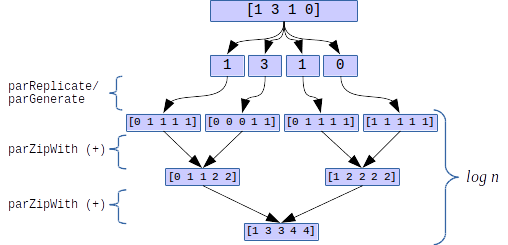
\includegraphics[width=\linewidth]{accuHist}
    \caption{Example execution of \c{accuHist [1,3,1,0]}}
    \label{fig:hist-org}
  \end{figure}

\section{Implementation}
  To implement \algo in parallel, we have to revisit our sequential
  implementation.
  
  It is fairly simple to integrate
  the parallel primitives into normalisation and scaling.
  However, \c{accuHist} and \c{apply} need to be adapted.
  
  \begin{lstlisting}
type Image  = Vector Int
type Hist   = Vector Int

hbalance :: Image -> Image
hbalance img =
  let hist = accuHist img
      min = hist ! 0
      max = hist ! gmax
      apply hist = parMap (\i -> h ! i) img
      sclNrm :: Int -> Int
      sclNrm x = floor ( (x-min)/(max - min)*gmax )
  in  apply (parMap sclNrm) hist

accuHist :: Image -> Hist
accuHist []  = parReplicate gmax 0
accuHist [x] =
  parGenerate gmax (\i -> if (i >= x) then 1 else 0)
accuHist xs  =
  let (left,right) = splitMid xs
      [leftRes,rightRes] = parMap accuHist [left,right]
  in  parZipWith (+) leftRes rightRes
  \end{lstlisting}
  
  The calculation of the parallel accumulated histogram calculation
  has been implemented as explained in the previous section.
  For the gray tone mapping (\c{apply}) to work, we cannot use nested arrays
  \footnote{As they would result into an array of pointers to subarrays.
  Due to Cache Locality, this is undesireable.}
  . We need to change our entire image representation to a flat array manually.
  To retrieve a specific pixel one needs to calculate
  the offset using the image's width. Fortunately,
  for \algo, we don't need to retrieve pixels by their indices anyways.
  However, the subsequent algorithms in the pipeline of image processing
  have to cope with this complication.

  ...
  USE COST-CENTRE PDF!
    
\section{Complexities}
  ...
